\begin{problem}
Calculate the quadratic polynomial that minimizes the expression
\begin{equation}
\max_i \lvert f (\xi_i) - p(\xi_i) \rvert, \quad p \in \mathcal{P}_2 
\end{equation}
for $f (x) = \lvert x - 1/2\rvert, x \in [0, 1]$ and the reference $\{0, 1/4, 1/2, 1\}$. Plot the function and its approximation. Plot the error function. Is this a best minimax approximation?
\end{problem}

\begin{solution}
We want to solve the equation system given by:
\begin{equation}
f(\xi_i) = \sum_{j=0}^n\left(\lambda_j\Phi_j(\xi)\right)+(-1)^ih
\label{thm74}
\end{equation}
We use the monomial basis $\{1,x,x^2\}$ and substituting our data in equation \ref{thm74} we get
\begin{equation}
f(\xi_i) = \lambda_0 + \lambda_1 \xi_i + \lambda_2 \xi_i^2 + (-1)^ih
\end{equation}
This leads to the system of equations:
\begin{align*}
\frac{1}{2} &= \lambda_0 + h \\
\frac{1}{4} &= \lambda_0 + \frac{\lambda_1}{4} + \frac{\lambda_2}{16} - h \\
0 &= \lambda_0 + \frac{\lambda_1}{2} + \frac{\lambda_2}{4} + h \\
\frac{1}{2} &= \lambda_0 + \frac{\lambda_1}{2} + \frac{\lambda_2}{4} - h
\end{align*}
Note that this system is always solvable as we know that the best approximation exists. Using MATLAB's \texttt{backslash} we obtain the solution $[0.5556, -1.8889, 1.7778, -0.0556]$ where the last element is $h$. Therefore we have that our polynomial is $p(x) = 0.5556 -1.8889x + 1.7778x^2$. As we can see in the Figure \ref{trialapprox} where we plot the function, the approximation and the error, this is not yet the best approximation.
\begin{figure}[h]
\centering 
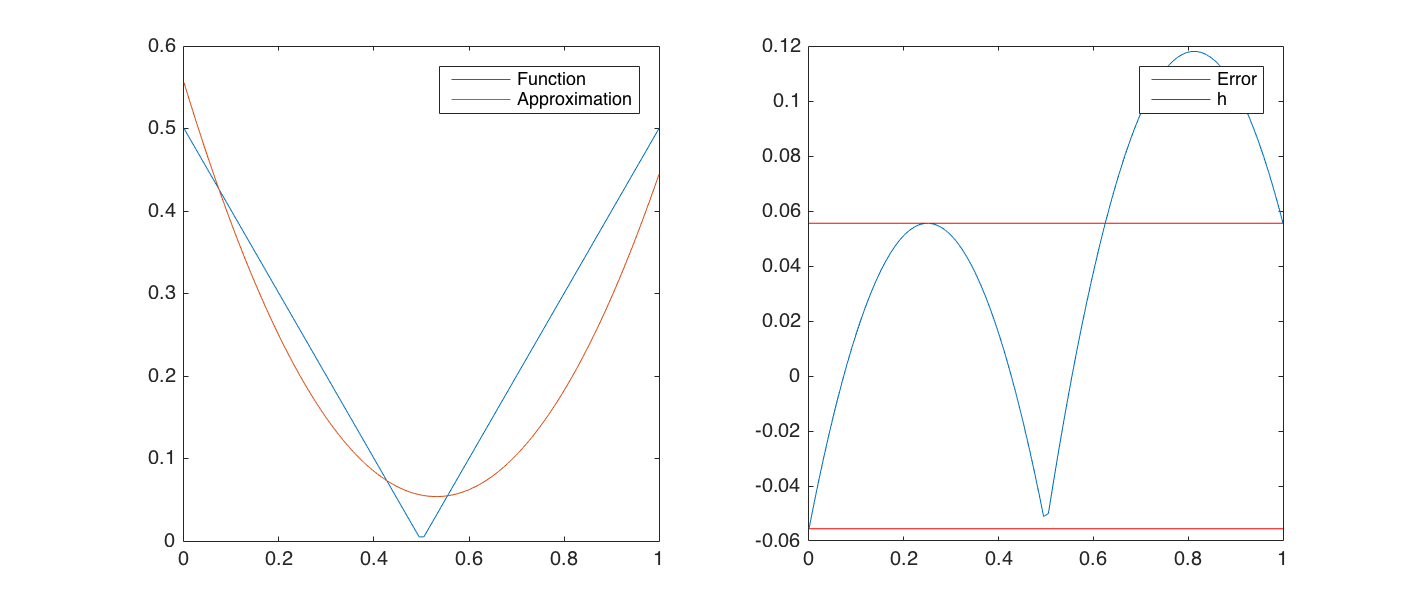
\includegraphics[scale = 0.25]{figtask2hwk4.png}
\caption{Function, approximation and error for the reference \{0, 1/4, 1/2, 1\}}
\label{trialapprox}
\end{figure}
To get a better result, we can take a step of the one point exchange algorithm. We can see that $\eta \approx 0.75$, therefore, following the algorithm (substitute $\eta$ with the $\xi$ that is closest and has the same sign), we have to change the reference to $\{0, 1/4, 1/2, 0.75\}$ obtaining the polynomial $p(x) = 0.5625 -2x+2x^2$ and the plots in Figure \ref{stepexchange}.
\begin{figure}[h]
\centering 
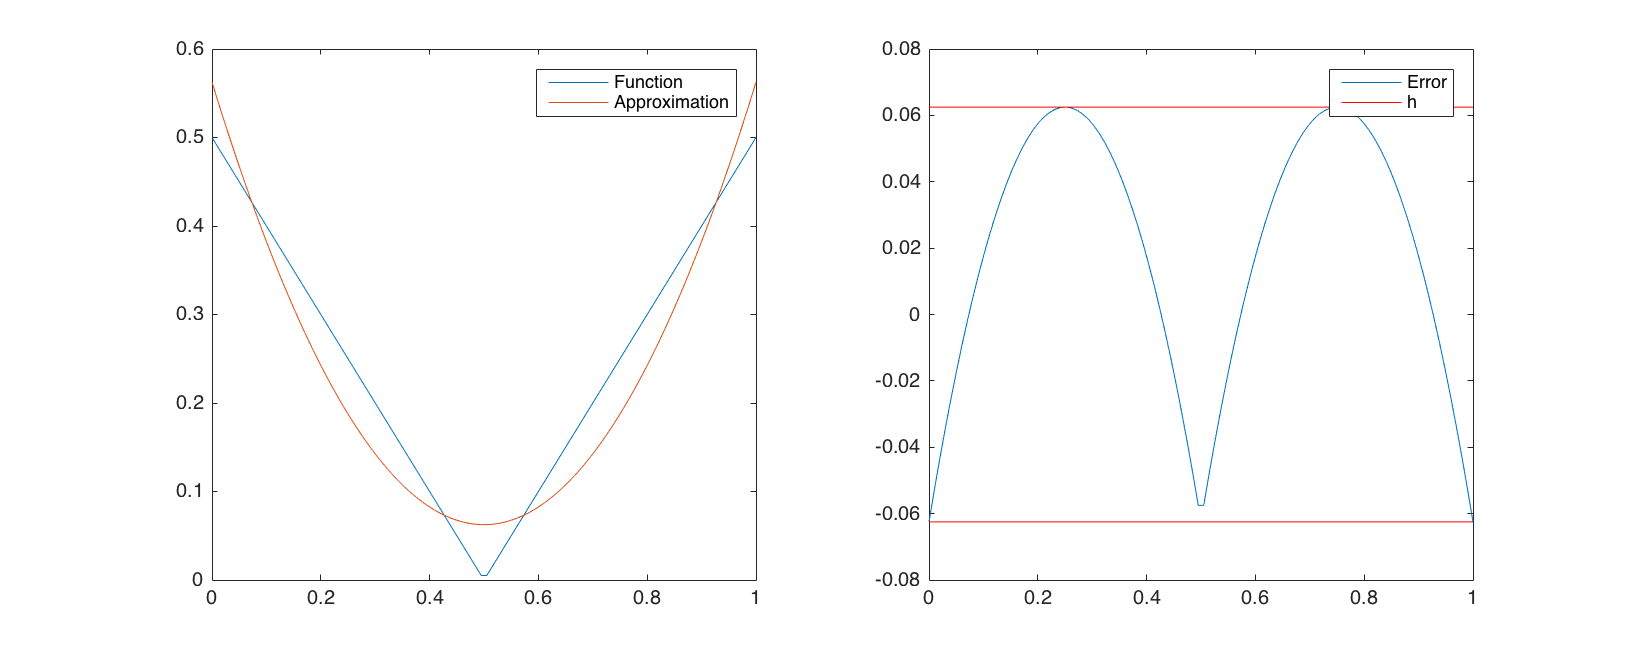
\includegraphics[scale = 0.25]{figtask2hwk4step1.png}
\caption{Function, approximation and error for the reference \{0, 1/4, 1/2, 0.75\}}
\label{stepexchange}
\end{figure}
Now this, if not the best approximation, is very close to what we would want in practice.
\end{solution}